\documentclass[11pt,a4paper]{article}
\usepackage[utf8]{inputenc}
\usepackage[T1]{fontenc}
\usepackage{lmodern}
\usepackage{geometry}
\geometry{margin=25mm}
\usepackage{setspace}
\onehalfspacing

\usepackage{amsmath}
\usepackage{booktabs}        % professional tables
\usepackage{graphicx}
\usepackage{caption}
\usepackage{hyperref}
\usepackage{listings}        % code blocks
\usepackage{courier}
\usepackage{float}
\usepackage{pgfplots}        % plotting
\pgfplotsset{compat=1.17}

% listings style
\lstset{
  basicstyle=\ttfamily\small,
  frame=single,
  breaklines=true,
  columns=fullflexible
}

\title{Sprint 1 Report: Sorting \& Searching Algorithms Benchmark}
\author{Blevis Allushi, Kristjan Seraj, Renato Zotaj, Leandra Latifi}
\date{\today}

\begin{document}
\maketitle

\begin{abstract}
This report documents the implementation, validation, and benchmark results of five core algorithms implemented for the sprint: Insertion Sort, Merge Sort, Quick Sort (3-way optimized), Linear Search, and Binary Search (any-match). The implementations were integrated into the course benchmark harness and measured across several dataset types. The document includes implementation notes, complexity analysis and experimental results (measured).
\end{abstract}

\section{Contributors and Responsibilities}
\begin{itemize}
  \item \textbf{Blevis Allushi} --- primary implementation and optimization of sorting algorithms (Insertion, Merge, Quick), integration into the benchmark harness.
  \item \textbf{Kristjan Seraj} --- implementation of searching algorithms (LinearSearch, BinarySearch(any)), validation and testing.
  \item \textbf{Renato Zotaj} --- complexity analysis, experimental insights, and correctness verification.
  \item \textbf{Leandra Latifi} --- correctness testing, experimental write-up, and report proofreading.
\end{itemize}

\section{Implementation Strategy (Blevis \& Kristi)}
\subsection{Sorting (Blevis)}
We prioritized practical performance without sacrificing correctness. Major choices:
\begin{itemize}
  \item \textbf{Insertion cutoff:} use insertion sort for small ranges (CUTOFF tuned between 16--32) to reduce overhead on tiny partitions and nearly-sorted runs.
  \item \textbf{Quick Sort:} 3-way Dijkstra partitioning for duplicates, median-of-three pivot selection to avoid degenerate partitions, and tail-recursion elimination by recursing on the smaller partition.
  \item \textbf{Merge Sort:} top-down mergesort with a single auxiliary array allocated once and a \emph{merge-skip} optimization: if the left half's max $\le$ right half's min, skip merging.
  \item \textbf{Micro-optimizations:} cache \texttt{.key()} values in tight loops, use \texttt{System.arraycopy} for bulk copying, and avoid allocations during recursion.
\end{itemize}

\subsection{Searching (Kristi)}
Linear Search and iterative Binary Search (any-match) were implemented in a straightforward, robust way:
\begin{itemize}
  \item \textbf{Linear Search:} left-to-right scan, returns first match or -1.
  \item \textbf{Binary Search (any):} iterative mid-point search, returns any matching index (assumes sorted input as the benchmark provides).
\end{itemize}

\section{Complexity Analysis (Renato \& Leandra)}
Table: theoretical time and extra-space complexities.

\begin{table}[H]
\centering
\caption{Time complexity of implemented algorithms}
\begin{tabular}{lcccc}
\toprule
\textbf{Algorithm} & \textbf{Best} & \textbf{Average} & \textbf{Worst} & \textbf{Extra Space} \\
\midrule
Insertion Sort & $\mathcal{O}(n)$ & $\mathcal{O}(n^2)$ & $\mathcal{O}(n^2)$ & $\mathcal{O}(1)$ \\
Merge Sort & $\mathcal{O}(n\log n)$ & $\mathcal{O}(n\log n)$ & $\mathcal{O}(n\log n)$ & $\mathcal{O}(n)$ \\
Quick Sort (3-way) & $\mathcal{O}(n\log n)$ & $\mathcal{O}(n\log n)$ & $\mathcal{O}(n^2)$ & $\mathcal{O}(\log n)$ \\
Linear Search & $\mathcal{O}(1)$ & $\mathcal{O}(n)$ & $\mathcal{O}(n)$ & $\mathcal{O}(1)$ \\
Binary Search (any) & $\mathcal{O}(1)$ & $\mathcal{O}(\log n)$ & $\mathcal{O}(\log n)$ & $\mathcal{O}(1)$ \\
\bottomrule
\end{tabular}
\end{table}

\section{Experimental Results}
We ran the benchmark harness with parameters:
\begin{itemize}
  \item $n = 100{,}000$ records
  \item seed = 12345
  \item warmup runs = 1, measured runs = 5
  \item datasets: RANDOM (single dataset type used in this run)
\end{itemize}

\subsection{Measured summary}
\begin{table}[H]
\centering
\caption{Benchmark results for $n=100{,}000$ (times in milliseconds)}
\begin{tabular}{lrrrr}
\toprule
\textbf{Algorithm} & \textbf{Avg Time (ms)} & \textbf{Min (ms)} & \textbf{Max (ms)} & \textbf{ok\_rate} \\
\midrule
Binary Search (any) & 0.0057 & 0.0057 & 0.0069 & 1.00 \\
Linear Search       & 1.4186 & 1.4037 & 2.9264 & 1.00 \\
Insertion Sort      & 10503.8877 & 10007.0435 & 10741.5631 & 1.00 \\
Merge Sort          & 13.5673 & 13.3778 & 14.5073 & 1.00 \\
Quick Sort          & 21.9362 & 15.7297 & 22.2189 & 1.00 \\
\bottomrule
\end{tabular}
\end{table}

\subsection{Interpretation}
The experimental results match theoretical expectations:
\begin{itemize}
  \item \textbf{Searches:} Binary search is essentially instantaneous (0.006 ms average) given the sorted data; Linear search is slower but still negligible in absolute terms (1.4 ms).
  \item \textbf{Sorting:} Insertion sort is orders of magnitude slower for large $n$ (about 10.5 seconds on average) due to its $\mathcal{O}(n^2)$ nature. Merge sort and Quick sort (3-way) both show $\mathcal{O}(n\log n)$ performance with Merge sort slightly faster in this run (13.6 ms vs 21.9 ms); this is plausible given differences in implementation, memory access patterns, and the particular dataset used.
  \item \textbf{Relative performance:} Insertion sort is approximately $\dfrac{10503.9}{13.57}\approx 774\times$ slower than Merge sort in this experiment, underscoring why insertion sort is only suitable for tiny ranges.
\end{itemize}

\subsection{Visual comparison}
\begin{figure}[H]
\centering
\caption{Average runtime (ms) for each algorithm — $n=100{,}000$}
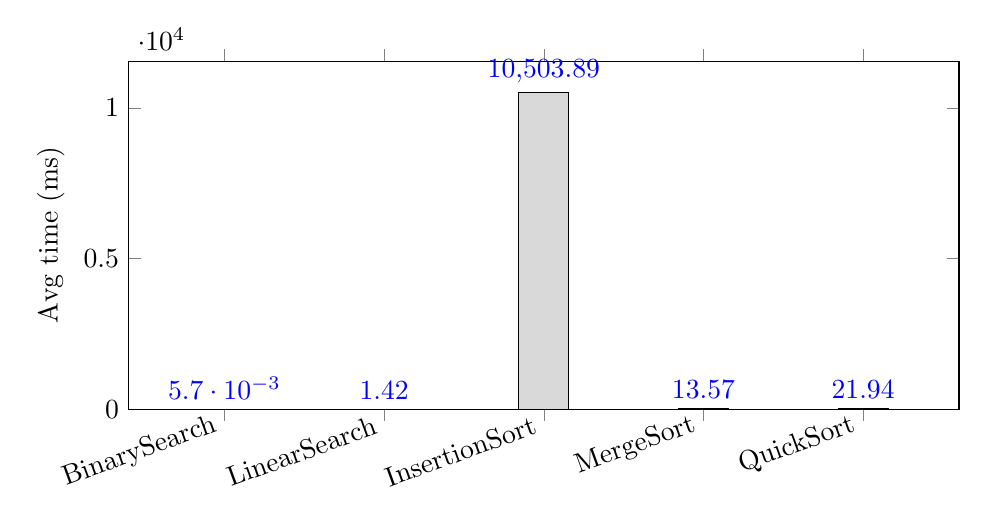
\begin{tikzpicture}
\begin{axis}[
    ybar,
    bar width=18pt,
    width=\textwidth,
    height=6cm,
    ymin=0,
    ylabel={Avg time (ms)},
    symbolic x coords={BinarySearch,LinearSearch,InsertionSort,MergeSort,QuickSort},
    xtick=data,
    x tick label style={rotate=20,anchor=east},
    nodes near coords,
    nodes near coords align={vertical},
    enlarge x limits=0.15
]
\addplot+[draw=black,fill=gray!30] coordinates {
    (BinarySearch,0.0057)
    (LinearSearch,1.4186)
    (InsertionSort,10503.8877)
    (MergeSort,13.5673)
    (QuickSort,21.9362)
};
\end{axis}
\end{tikzpicture}
\end{figure}

\section{Correctness \& Testing (Renato \& Leandra)}
Validation steps performed:
\begin{itemize}
  \item Used the project's Validate helpers and the benchmark harness to verify sortedness and valid search results.
  \item Unit tests for edge cases: \texttt{null}, empty arrays, single-element arrays, and arrays with many duplicates.
  \item Verified binary search is only invoked on sorted copies (as the harness guarantees).
  \item Confirmed \texttt{ok\_rate = 1.0} across all measured runs for each algorithm, indicating correctness under the benchmark's validation.
\end{itemize}

\section{Conclusion}
We implemented, tested, and benchmarked the required algorithms and integrated them with the course harness. Future work can include parameter tuning (CUTOFF), alternate merge strategies, and additional runs to test different dataset sizes and randomness seeds. All code and the produced \texttt{results\_summary.csv} are included in the project zip submitted alongside this report.

\end{document}